\documentclass{minimal}
\usepackage{graphicx,color}
\usepackage[utf8]{inputenc}
\usepackage[papersize={420.00bp,315.00bp},text={420.00bp,315.00bp}]{geometry}
\begin{document}
\centering
% Title: gl2ps_renderer figure
% Creator: GL2PS 1.4.2, (C) 1999-2020 C. Geuzaine
% For: Octave
% CreationDate: Mon Dec 12 15:58:18 2022
\setlength{\unitlength}{1pt}
\begin{picture}(0,0)
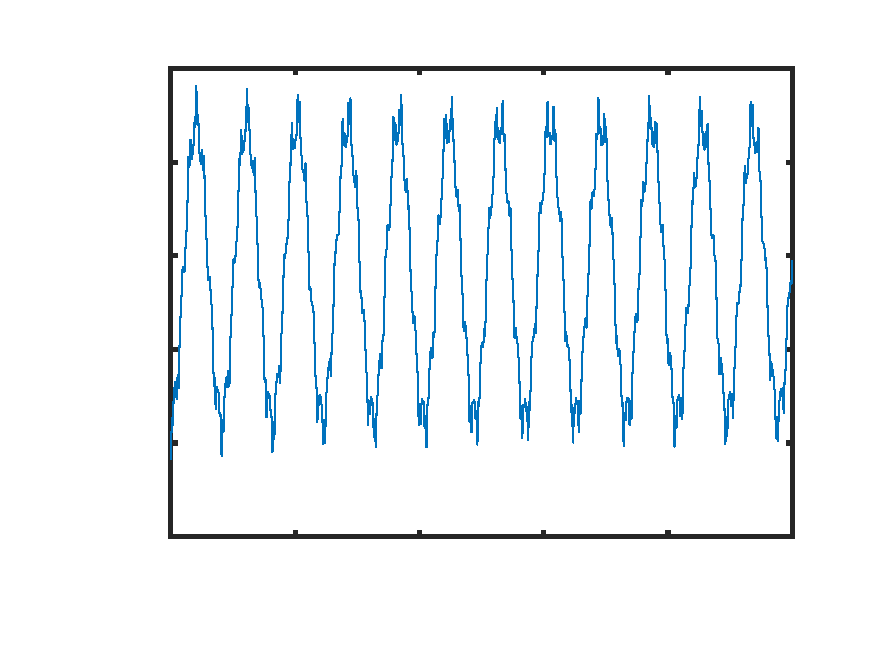
\includegraphics[scale=1]{DoubleKapitzaTimeSeriesTheta1-inc}
\end{picture}%
\begin{picture}(420,315)(0,0)
\fontsize{22}{0}\selectfont\put(82.0095,40.8621){\makebox(0,0)[t]{\textcolor[rgb]{0.15,0.15,0.15}{{0}}}}
\fontsize{22}{0}\selectfont\put(141.661,40.8621){\makebox(0,0)[t]{\textcolor[rgb]{0.15,0.15,0.15}{{20}}}}
\fontsize{22}{0}\selectfont\put(201.312,40.8621){\makebox(0,0)[t]{\textcolor[rgb]{0.15,0.15,0.15}{{40}}}}
\fontsize{22}{0}\selectfont\put(260.964,40.8621){\makebox(0,0)[t]{\textcolor[rgb]{0.15,0.15,0.15}{{60}}}}
\fontsize{22}{0}\selectfont\put(320.615,40.8621){\makebox(0,0)[t]{\textcolor[rgb]{0.15,0.15,0.15}{{80}}}}
\fontsize{22}{0}\selectfont\put(380.266,40.8621){\makebox(0,0)[t]{\textcolor[rgb]{0.15,0.15,0.15}{{100}}}}
\fontsize{22}{0}\selectfont\put(71,57.3375){\makebox(0,0)[r]{\textcolor[rgb]{0.15,0.15,0.15}{{3}}}}
\fontsize{22}{0}\selectfont\put(71,102.27){\makebox(0,0)[r]{\textcolor[rgb]{0.15,0.15,0.15}{{3.05}}}}
\fontsize{22}{0}\selectfont\put(71,147.202){\makebox(0,0)[r]{\textcolor[rgb]{0.15,0.15,0.15}{{3.1}}}}
\fontsize{22}{0}\selectfont\put(71,192.135){\makebox(0,0)[r]{\textcolor[rgb]{0.15,0.15,0.15}{{3.15}}}}
\fontsize{22}{0}\selectfont\put(71,237.068){\makebox(0,0)[r]{\textcolor[rgb]{0.15,0.15,0.15}{{3.2}}}}
\fontsize{22}{0}\selectfont\put(71,282){\makebox(0,0)[r]{\textcolor[rgb]{0.15,0.15,0.15}{{3.25}}}}
\fontsize{24}{0}\selectfont\put(231.138,18.8622){\makebox(0,0)[t]{\textcolor[rgb]{0.15,0.15,0.15}{{Time}}}}
\fontsize{24}{0}\selectfont\put(24,169.669){\rotatebox{90}{\makebox(0,0)[b]{\textcolor[rgb]{0.15,0.15,0.15}{{$\theta_1$}}}}}
\fontsize{24}{0}\selectfont\put(231.138,292){\makebox(0,0)[b]{\textcolor[rgb]{0,0,0}{{Time Series of $\theta_1$}}}}
\end{picture}
\end{document}
